Este capítulo mapeia sistematicamente as pesquisas existentes na interseção entre Inteligência Artificial e dados parlamentares, com o objetivo de identificar o que já foi feito, onde estão as lacunas, e como este trabalho se posiciona em relação à literatura.

Optou-se pelo Mapeamento Sistemático da Literatura (MSL) em vez de uma revisão narrativa porque o escopo do tema é amplo e interdisciplinar — abrangendo PLN, dados abertos, transparência governamental e interação humano-dados —, o que exige um protocolo estruturado para evitar seleção tendenciosa de fontes \cite{Kitchenham2004}. A diferença entre MSL e revisão sistemática é relevante aqui: enquanto a revisão sistemática busca sintetizar evidências sobre uma intervenção específica, o mapeamento tem por objetivo caracterizar o espaço de pesquisa, identificar tendências e delimitar lacunas, o que é mais adequado para áreas emergentes como a aplicação de IA Generativa em contextos legislativos \cite{Kitchenham2004}.

O protocolo seguiu as diretrizes de Kitchenham \cite{Kitchenham2004}, estruturado em três fases: Planejamento, Execução e Análise.

\section{Protocolo do Mapeamento Sistemático}

O processo adotado seguiu as três fases críticas recomendadas pela literatura: Planejamento, Execução e Análise. Tal abordagem estruturada assegura o rigor na seleção dos estudos. A Figura \ref{fig:fase_rsl} ilustra o fluxo de trabalho.

\begin{figure}[H]
    \centering
    \caption{Fases do Mapeamento Sistemático da Literatura}
    \label{fig:fase_rsl}
    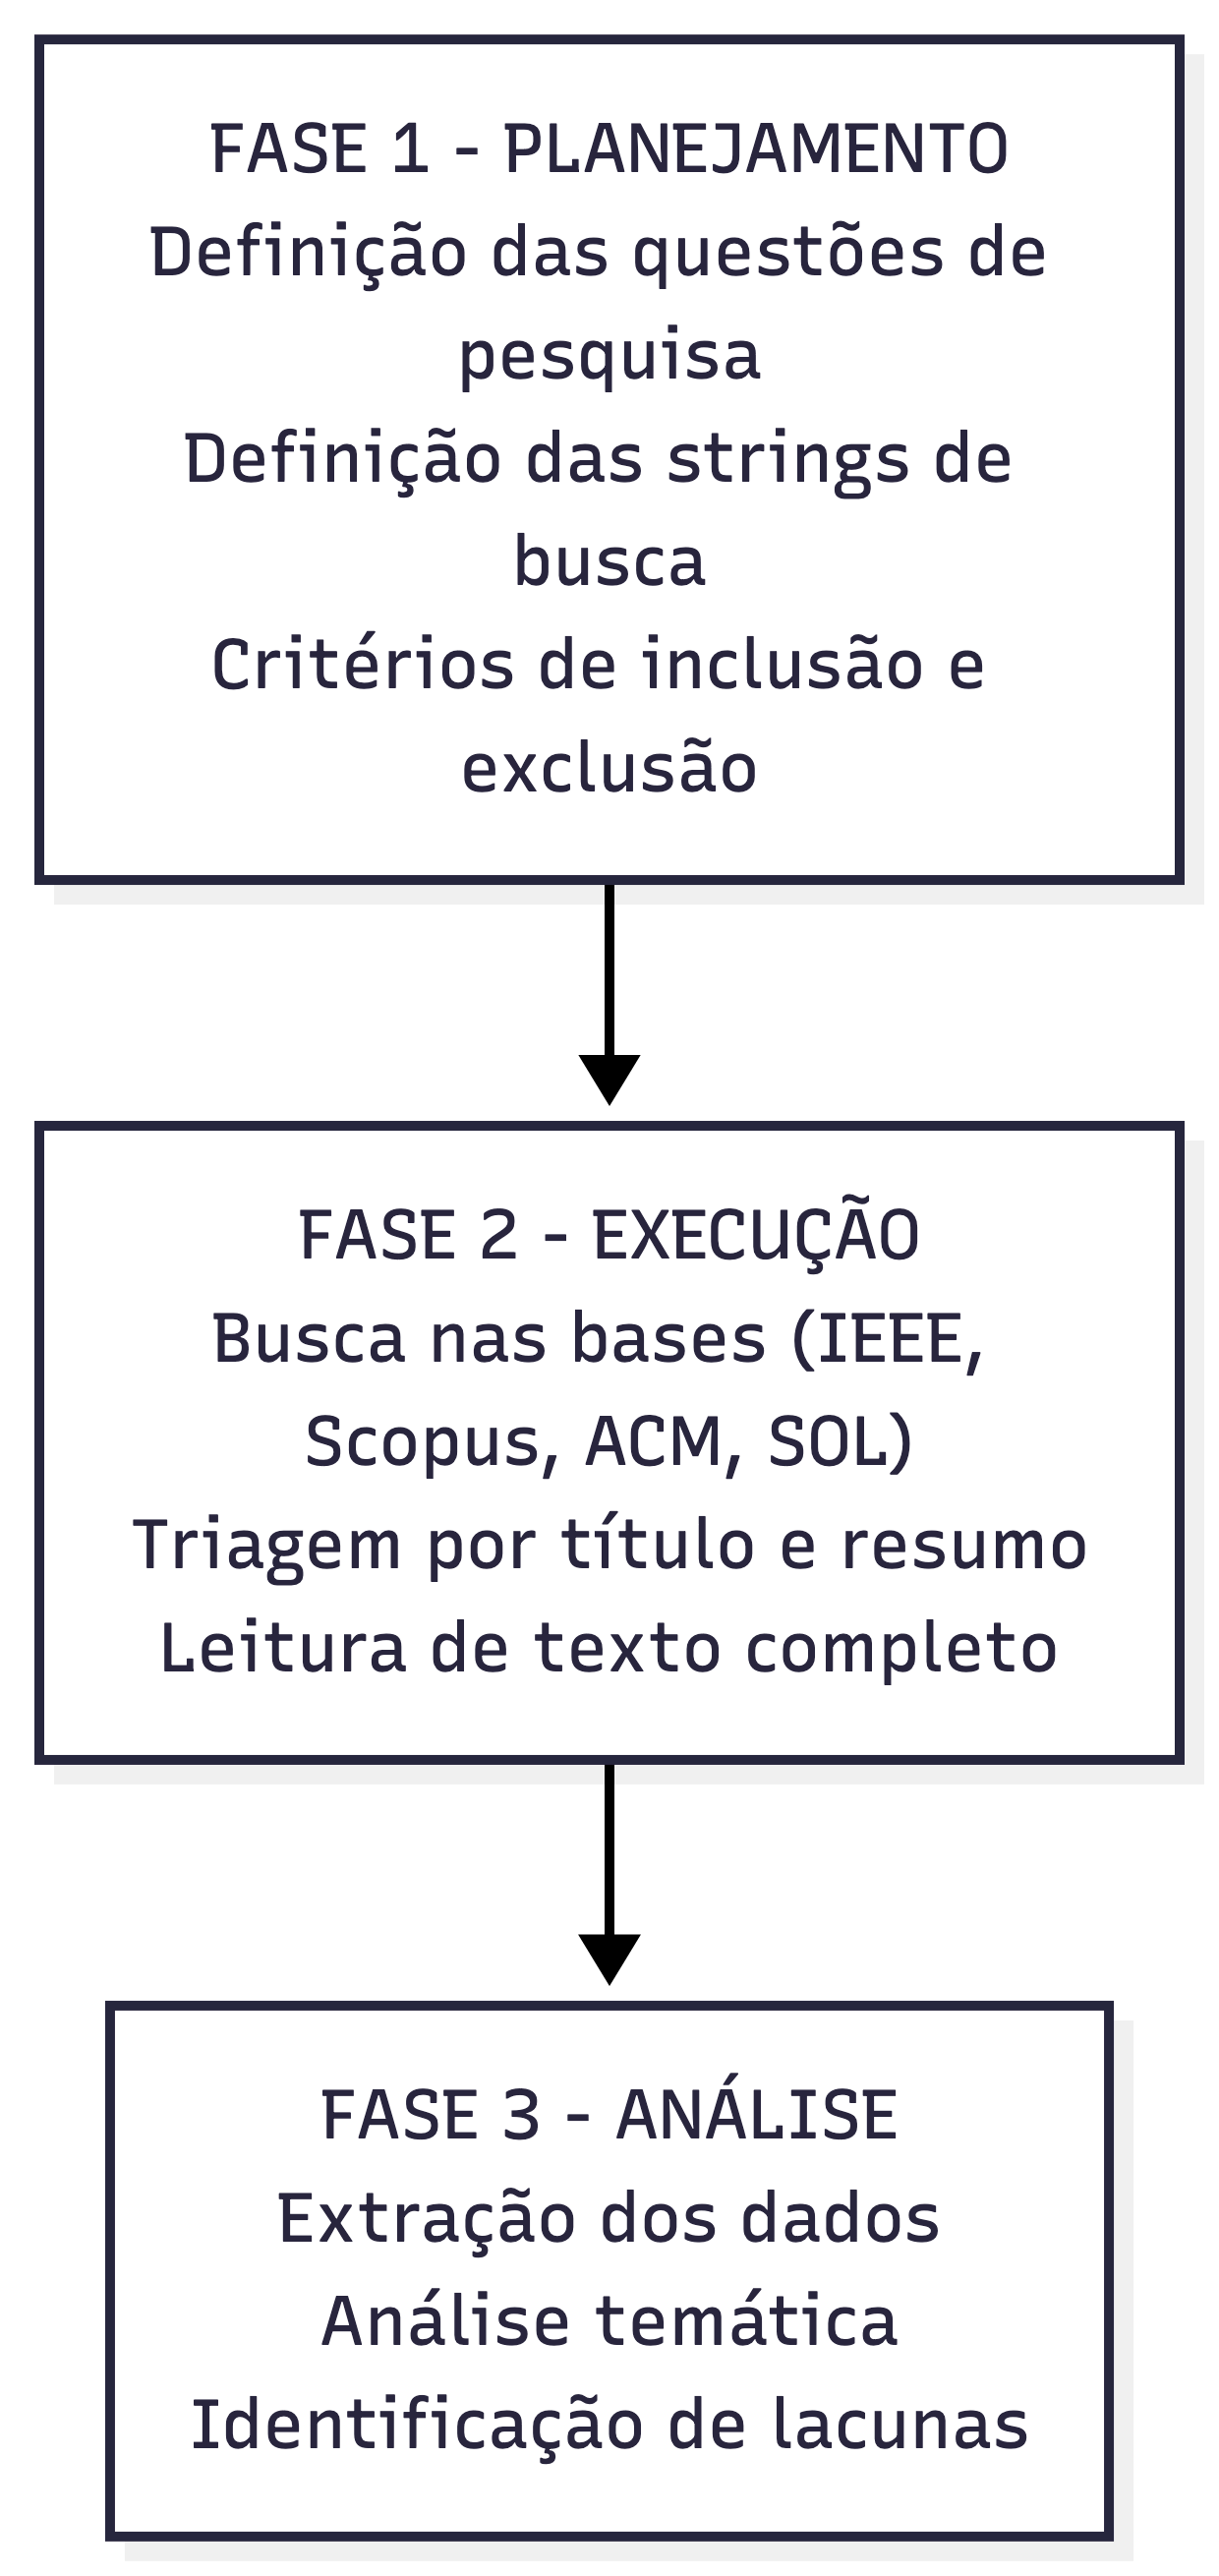
\includegraphics[width=0.5\textwidth]{imagens/fase_rsl.png}
    \fonte{Adaptado de Kitchenham (2004).}
\end{figure}

Para a organização e condução do mapeamento, utilizou-se a ferramenta \textit{Parsifal}\footnote{\url{https://parsif.al/}}, que oferece suporte computacional para a aplicação dos critérios de seleção e extração de dados.

\subsection{Planejamento}

Nesta etapa, definiu-se a necessidade do mapeamento e o protocolo de pesquisa \cite{Brereton2007}. O objetivo central foi responder às questões de pesquisa detalhadas no Quadro \ref{tab:questoes_pesquisa}, que orientaram a estratégia de busca.

\begin{quadro}[H]
    \centering
    \caption{Questões de Pesquisa do Mapeamento Sistemático}
    \label{tab:questoes_pesquisa}
    \begin{tabular}{p{3cm}p{10cm}}
    \toprule
    \textbf{ID da Questão} & \textbf{Questões de Pesquisa} \\
    \midrule
    Q1: & Quais técnicas de Inteligência Artificial ou PLN são mais utilizadas na literatura para a análise de dados parlamentares abertos? \\
    Q2: & Existem trabalhos que aplicam IA Generativa (LLMs) ou interfaces conversacionais (\textit{chatbots}) para facilitar o acesso do cidadão a dados legislativos? \\
    Q3: & Quais são as principais lacunas e desafios apontados pela literatura na democratização do acesso à informação parlamentar? \\
    Q4: & Como a literatura trata interação humano-dados e acessibilidade de informação legislativa? \\
    \bottomrule
    \end{tabular}
    \fonte{Produção da autora.}
\end{quadro}

Para responder a essas questões, foram definidos os campos de extração apresentados no Quadro \ref{tab:campo_extracao}.

\begin{quadro}[H]
    \centering
    \caption{Campos de Extração de Dados}
    \label{tab:campo_extracao}
    \begin{tabular}{p{10cm}}
    \toprule
    \textbf{Campo de Extração} \\
    \midrule
    Ano de Publicação \\
    Técnica/Método de IA/PLN Utilizado \\
    Uso de IA Generativa ou \textit{Chatbot}? \\
    Contexto Legislativo (Nacional vs. Internacional) \\
    Enfoque em Acessibilidade ou Interação Humano-Dados \\
    Desafios/Lacunas Identificados \\
    \bottomrule
    \end{tabular}
    \fonte{Produção da autora.}
\end{quadro}

\textbf{Fontes de Busca:}

Para esta pesquisa, a busca foi conduzida em cinco bases de dados de alto impacto internacional e nacional:

\begin{itemize}
    \item \textbf{IEEE Xplore:} Base multidisciplinar de Engenharia e Computação
    \item \textbf{Scopus:} Indexador de citações com cobertura de múltiplas disciplinas
    \item \textbf{ACM Digital Library:} Publicações especializadas em Ciência da Computação
    \item \textbf{Web of Science (WoS):} Base multidisciplinar de alto fator de impacto, incluída para ampliar a cobertura de publicações internacionais em Ciências da Computação e Sistemas de Informação
    \item \textbf{SOL - Biblioteca Digital da SBC:} Repositório da Sociedade Brasileira de Computação (\url{https://sol.sbc.org.br/}) para capturar produção científica nacional relevante
\end{itemize}

O escopo temporal compreendeu o período de 2014 a 2026, refletindo a evolução das políticas de dados abertos no Brasil e a emergência recente de aplicações baseadas em IA Generativa.

Data da busca: Maio de 2026.

As palavras-chave e \textit{strings} de busca utilizadas estão detalhadas nos Quadros \ref{tab:palavras_chave} e \ref{tab:string_busca}.

\begin{quadro}[H]
    \centering
    \caption{Palavras-Chave da Busca}
    \label{tab:palavras_chave}
    \begin{tabular}{p{5cm}p{8cm}}
    \toprule
    \textbf{Palavras-Chave (PT)} & \textbf{Termos em Inglês} \\
    \midrule
    Dados Parlamentares & Parliamentary Data, Legislative Data, Plenary Sessions \\
    IA Generativa & Generative Artificial Intelligence, LLM, Large Language Models \\
    Análise de Discursos & Information Extraction, Text Analysis, Speech Mining \\
    Dados Abertos & Open Government Data, Open Data \\
    Interface Conversacional & Chatbot, Conversational AI, Dialog Systems \\
    Acessibilidade de Dados & Data Accessibility, Data Literacy \\
    Transparência Legislativa & Legislative Transparency, Open Parliament \\
    \bottomrule
    \end{tabular}
    \fonte{Produção da autora.}
\end{quadro}

\begin{quadro}[H]
    \centering
    \caption{Strings de Busca (Conceituais)}
    \label{tab:string_busca}
    \begin{tabular}{p{13cm}}
    \toprule
    \textbf{String de Busca} \\
    \midrule
    (``Parliamentary Data" OR ``Legislative Data") AND (``Generative AI" OR ``Large Language Models" OR ``LLM" OR ``Chatbot") \\
    (``Open Government Data") AND (``Natural Language Processing" OR ``NLP" OR ``Text Mining") AND (``Parliament" OR ``Legislature") \\
    (``Legislative Transparency") AND (``Artificial Intelligence" OR ``Machine Learning") \\
    (``Data Accessibility") AND (``Chatbot" OR ``Conversational AI") \\
    \bottomrule
    \end{tabular}
    \fonte{Produção da autora.}
\end{quadro}

O Quadro \ref{tab:criterios} apresenta os critérios estabelecidos para filtrar os trabalhos.

\begin{quadro}[H]
    \centering
    \caption{Critérios de Inclusão e Exclusão}
    \label{tab:criterios}
    \begin{tabular}{p{6.5cm}p{6.5cm}}
    \toprule
    \textbf{Critérios de Inclusão} & \textbf{Critérios de Exclusão} \\
    \midrule
    CI1: Aborda IA/PLN/LLM para dados governamentais ou parlamentares. & CE1: Estudos duplicados em múltiplas bases. \\
    CI2: Discute transparência ou participação política em contexto legislativo. & CE2: Literatura cinzenta ou não revisada por pares. \\
    CI3: Aborda dados abertos em contexto público/legislativo. & CE3: Estudos secundários (revisões de revisões). \\
    CI4: Investiga interação humano-dados ou acessibilidade. & CE4: Artigos que abordam exclusivamente aspectos legais/políticos sem componente técnico. \\
    \bottomrule
    \end{tabular}
    \fonte{Produção da autora.}
\end{quadro}

\subsection{Execução e Resultados}

A execução seguiu o protocolo estabelecido, compreendendo identificação, seleção, elegibilidade e inclusão. A busca inicial nas cinco bases retornou 47 estudos: IEEE Xplore (0), Scopus (6), ACM Digital Library (39), Web of Science (2) e SOL/SBC (0). A ausência de retorno na SOL/SBC e no IEEE para as \textit{strings} aplicadas foi registrada como resultado negativo esperado — dado o recorte temporal e temático definido — e não implica ausência de produção nacional na área. Após remoção de 2 duplicatas e aplicação dos critérios de inclusão/exclusão (triagem por título e resumo, seguida de leitura de texto completo), selecionaram-se 7 trabalhos primários como mais relevantes para contextualizar esta dissertação.

O fluxo de seleção é detalhado na Figura \ref{fig:fluxograma_execucao}.

\begin{figure}[H]
    \centering
    \caption{Fluxograma de seleção dos estudos (PRISMA-ScR)}
    \label{fig:fluxograma_execucao}
    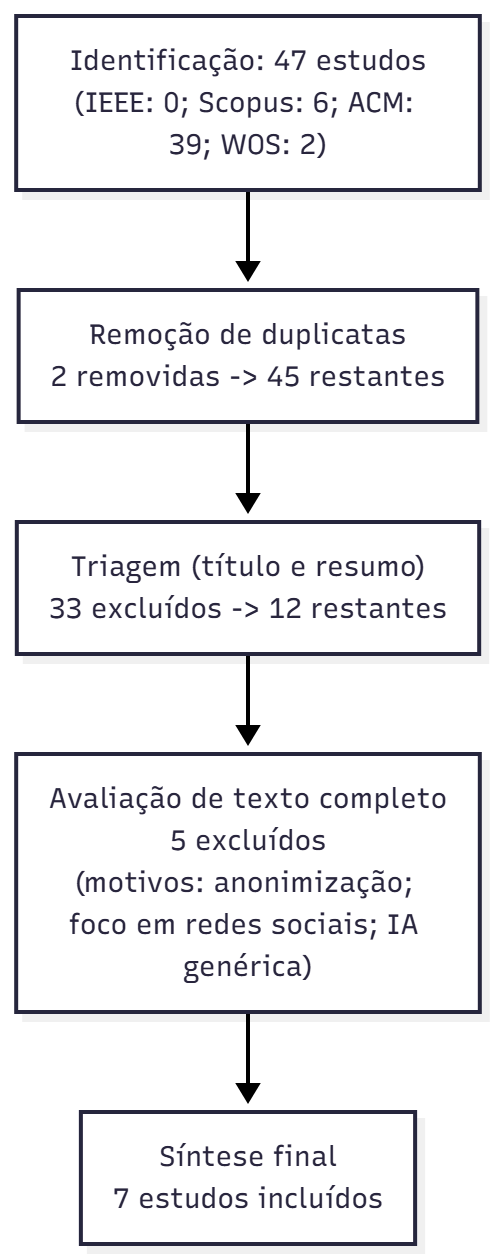
\includegraphics[width=0.5\textwidth]{imagens/fluxograma_execucao.png}
    \fonte{Produção da autora.}
\end{figure}

\section{Análise Temática dos Resultados}

Diferentemente de uma mera listagem de resumos, a análise temática busca identificar padrões, convergências e divergências entre os trabalhos, conectando-os explicitamente aos objetivos desta pesquisa e às lacunas identificadas.

\subsection{Tema 1: IA Generativa para Estruturação de Dados Legislativos}

Os trabalhos de Colombo et al. (2025), Colombo (2024) e Von Lucke e Frank (2025) convergem em um ponto fundamental: \textbf{modelos de linguagem generativa conseguem, quando bem orientados, transformar dados legislativos complexos em estruturas de conhecimento compreensíveis}.

\textbf{Especificidades de cada trabalho:}

\begin{itemize}
    \item \citeonline{Colombo2025} propõem um \textit{pipeline} assistido por LLM para construção automática de \textit{knowledge graphs} da legislação italiana. O trabalho demonstra que IA pode extrair entidades jurídicas (leis, artigos, interpretações) de textos legislativos não estruturados e organizá-las em grafos semânticos. Limitação: foca em estruturação técnica, não em acessibilidade para cidadãos.

    \item \citeonline{Colombo2024} aprofunda a discussão anterior, explorando explicitamente a sinergia entre grafos de conhecimento e LLMs para \textit{monitoring} de sistemas legislativos — rastreamento de como leis evoluem. Contribuição: metodologia de versionamento de legislação.

    \item \citeonline{VonLuckeFrank2025} analisam a aplicação prática de ferramentas como ChatGPT em parlamentos, levantando questões críticas sobre potencialidades (rapidez, síntese) e riscos (alucinação, imprecisão factual). Este trabalho é particularmente relevante pois trata de LLMs em contexto parlamentar e aponta desafios de confiabilidade.
\end{itemize}

\textbf{Padrão Emergente:} LLMs conseguem estruturar legislação, mas confiabilidade das respostas é crítica. A literatura aponta a necessidade de validação humana.

\textbf{Conexão com Este Trabalho:} Esta pesquisa avança ao (1) avaliar tecnicamente a confiabilidade das respostas geradas, (2) combinar estruturação de dados com interfaces visual e conversacional, (3) focar em dados parlamentares brasileiros.

\subsection{Tema 2: Interfaces Conversacionais para Acessibilidade}

\citeonline{Kim2025} descrevem o ``LegisFlow", uma interface conversacional com ``consciência temporal" para pesquisa jurídica na Coreia. Este trabalho é diretamente alinhado aos objetivos desta dissertação.

\textbf{Especificidades:}

\begin{itemize}
    \item Implementa chatbot para consultas em linguagem natural sobre legislação
    \item Incorpora noção de tempo (como leis mudaram ao longo do tempo)
    \item Avalia usabilidade com usuários reais
    \item Contexto: público coreano sem expertise jurídica
\end{itemize}

\textbf{Padrão Emergente:} Interfaces conversacionais reduzem barreira de entrada para acesso legislativo. Dimensão temporal é importante.

\textbf{Conexão e Diferenciação:} Este trabalho dialoga com o LegisFlow, mas dele se distingue deliberadamente. A interface conversacional, em si, não é a contribuição reivindicada --- ela já é demonstrada por Kim et al., inclusive com avaliação junto a usuários reais. O diferencial desta dissertação assenta-se em três eixos: (i) o contexto brasileiro e a língua portuguesa, ausentes naquele trabalho; (ii) a combinação de \textit{dashboard} visual e agente conversacional em um mesmo artefato, atendendo a padrões de uso distintos; e (iii) o foco explícito na rastreabilidade técnica das respostas, com instrumentação e métricas próprias, em vez da usabilidade percebida. Reconhece-se, em contrapartida, que este trabalho não avalia o impacto junto a usuários reais --- dimensão em que o LegisFlow avança e que aqui se delimita como trabalho futuro.

\subsection{Tema 3: Análise de Dados Legislativos com PLN Clássico}

\citeonline{Mendes2025} utilizam \textit{Topic Modeling} (técnica clássica de PLN, não IA Generativa) para analisar Pedidos de Acesso à Informação brasileiros. \citeonline{Bojars2019} apresentam ``LinkedSaeima", um dataset de dados abertos conectados (\textit{Linked Data}) do parlamento da Letônia.

\textbf{Padrão Emergente:} Abordagens clássicas de PLN conseguem extrair insights, mas requerem expertise técnica. IA Generativa oferece potencial para democratizar acesso.

\textbf{Conexão com Este Trabalho:} Enquanto esses trabalhos usam técnicas sofisticadas (Topic Modeling, RDF/Linked Data), o foco desta pesquisa é em acessibilidade para cidadãos não-especialistas. Essa é a lacuna que esta dissertação endereça.

\subsection{Tema 4: Desafios e Lacunas na Literatura}

\citeonline{PapadopoulosCharalabidis2020} aplicam PLN para extrair \textit{insights} de documentos de estratégias nacionais de IA, focando em mineração de textos governamentais. O trabalho, embora não focado em legislação, aponta desafios gerais na análise de textos públicos.

\textbf{Lacunas Identificadas Pela Literatura:}

\begin{enumerate}
    \item \textbf{Falta de foco em acessibilidade para cidadãos:} A maioria dos trabalhos trata estruturação técnica ou análise especializada, não democratização de acesso.

    \item \textbf{Confiabilidade de LLMs não é plenamente abordada:} Von Lucke e Frank apontam riscos, mas nenhum trabalho apresenta estratégia sistemática de validação.

    \item \textbf{Contexto brasileiro pouco explorado:} Dos 7 trabalhos, apenas Mendes et al. e Bojārs et al. abordam contexto nacional (coreano, letão, brasileiro). Falta pesquisa em português sobre legislação brasileira com IA Generativa.

    \item \textbf{Avaliação de respostas e rastreabilidade ainda é pouco explorada:} A literatura aponta riscos de alucinação e imprecisão factual em LLMs, mas ainda há espaço para protocolos de avaliação voltados à coerência entre respostas geradas e dados legislativos de origem.

    \item \textbf{Combinação Dashboard + Chatbot não é explorada:} Trabalhos tratam uma ou outra modalidade, raramente ambas integradas.
\end{enumerate}

\section{Lacunas Identificadas e Contribuições Desta Pesquisa}

Com base na análise sistemática, identificam-se as seguintes lacunas que esta pesquisa propõe-se a preencher:

\begin{enumerate}
    \item \textbf{Lacuna 1: Falta de foco em acessibilidade para cidadãos não-especialistas}
    \begin{itemize}
        \item \textbf{O que a literatura oferece:} Técnicas sofisticadas de IA para estruturação de legislação
        \item \textbf{O que está faltando:} Investigação de como essas técnicas podem ser comunicadas de forma compreensível ao cidadão médio
        \item \textbf{Como esta pesquisa aborda:} Design deliberado de interfaces acessíveis (Dashboard + Chatbot) e avaliação técnica de sua capacidade de organizar e consultar dados parlamentares
    \end{itemize}

    \item \textbf{Lacuna 2: Confiabilidade e validação de respostas IA não é sistemática}
    \begin{itemize}
        \item \textbf{O que a literatura oferece:} Identificação de riscos (alucinação, imprecisão)
        \item \textbf{O que está faltando:} Metodologia sistemática de validação antes de deploy em contexto cívico
        \item \textbf{Como esta pesquisa aborda:} Avaliação técnica rigorosa por meio de comparação com gabarito de referência, análise factual das respostas e verificação de rastreabilidade
    \end{itemize}

    \item \textbf{Lacuna 3: Contexto e idioma brasileiros pouco explorados}
    \begin{itemize}
        \item \textbf{O que a literatura oferece:} Exemplos internacionais (Itália, Coreia, Letônia)
        \item \textbf{O que está faltando:} Pesquisa em português sobre Senado Federal brasileiro
        \item \textbf{Como esta pesquisa aborda:} Dados reais da API do Senado Federal, legislação e dados parlamentares em língua portuguesa, contexto brasileiro até então ausente na literatura
    \end{itemize}

    \item \textbf{Lacuna 4: Avaliação factual e rastreável de respostas em linguagem natural}
    \begin{itemize}
        \item \textbf{O que a literatura oferece:} Discussões sobre potencial de LLMs e riscos de imprecisão
        \item \textbf{O que está faltando:} Protocolos explícitos para verificar se respostas geradas estão ancoradas em dados legislativos oficiais
        \item \textbf{Como esta pesquisa aborda:} Avaliação das respostas do AgentAI por cenários de consulta, comparação com dados oficiais e análise de rastreabilidade
    \end{itemize}

    \item \textbf{Lacuna 5: Integração de múltiplas modalidades de interação}
    \begin{itemize}
        \item \textbf{O que a literatura oferece:} Dashboards OU Chatbots, raramente ambos
        \item \textbf{O que está faltando:} Investigação de como diferentes modalidades se complementam para diferentes usuários
        \item \textbf{Como esta pesquisa aborda:} Design deliberado de Dashboard + Chatbot com avaliação de como ambos contribuem ao acesso democrático
    \end{itemize}
\end{enumerate}

\section{Conclusões do Mapeamento Sistemático}

O mapeamento revela um campo em formação: trabalhos sobre IA Generativa aplicada a legislação são recentes (predominantemente pós-2022), concentrados em contextos europeus e asiáticos, e orientados predominantemente à estruturação técnica — não à acessibilidade para cidadãos comuns. A ausência de trabalhos em português sobre dados parlamentares brasileiros com LLMs, combinada à falta de protocolos sistemáticos para avaliação de rastreabilidade e qualidade factual de respostas geradas, configura o espaço em que esta dissertação se insere.

É importante registrar uma limitação do próprio mapeamento: o corpus de 7 estudos primários selecionados é pequeno para afirmações categóricas sobre o estado da área, e a forte concentração de retornos em uma única base (ACM Digital Library) pode enviesar as lacunas identificadas, que devem, portanto, ser lidas como indícios e não como conclusões definitivas. Essa limitação pode refletir tanto a emergência da temática quanto restrições das \textit{strings} de busca utilizadas. A reexecução conduzida na RSL desta dissertação ampliou o escopo de bases consultadas e documentou, em apêndice, as \textit{strings} exatas aplicadas em cada base, com os respectivos números de retorno e filtros --- requisitos para a plena reprodutibilidade, conforme as diretrizes de Kitchenham \cite{Kitchenham2004}. A complementação por \textit{snowballing} --- para frente e para trás --- a partir dos estudos incluídos não foi conduzida nesta versão e fica registrada como trabalho futuro.
